% Graduation documentation
% Copyright 2016-2017, Sjors van Gelderen

% Document settings
\documentclass{article}
\author{Sjors van Gelderen}
\title{Exploring advanced programming concepts}
\date{\today{}}

% Packages
\usepackage{amsmath}
\usepackage[utf8]{inputenc}
\usepackage{listings}
\usepackage{float}
\usepackage{graphicx}
\graphicspath{{images/}}

% Content
\begin{document}

\maketitle{}

\newpage

\tableofcontents{}


\newpage


\section{Introduction}
In this document I describe the materials studied during my graduation phase.
The aim of the project was to prepare for professionally teaching students selective aspects of computer science.
These aspects include:
\begin{itemize}
\item{The C\# and Python 3 programming languages}
\item{Object-oriented design patterns}
\item{Data structures, algorithms and complexity analysis}
\end{itemize}

% ATTENTION REQUIRED: MISSING EXPLANATION
% ATTENTION REQUIRED: MISSING REPOSITORY LOCATION
\paragraph{}
I have provided many example implementations in a variety of programming languages.
All provided complexities in this document and related implementations are worst-case complexities.

\subsection{Primary languages}
Here is a brief description of the main languages used.

\subsubsection{C\#}
% ATTENTION REQUIRED: CITATION NEEDED
C\# is Microsoft's most popular .NET programming language.
The language strikes me as a much higher level variant of C++.
With its rich .NET ecosystem, modern features (LINQ, anonymous methods, tasks, etcetera),
C\# is certainly a powerful programming language.

\paragraph{Sources}
C\# code is provided in the subdirectory {\em csharp/}.

\subsubsection{Python 3}
Advantages of this language include its concise syntax and its portability.
Because of Python 3's high-level nature, the programmer can focus exclusively on the actual logic of an algorithm,
rather than the low-level memory management involved. This is removes a significant source of potential distraction.
Unfortunately, the absence of a strict compiler means frequent run-time debugging sessions are necessary.

\paragraph{Sources}
Python 3 code is provided in the subdirectory {\em python\_3/}.

\subsubsection{F\#}
% ATTENTION REQUIRED: CITATION NEEDED
Being a more recent addition to the .NET family of programming languages,
F\# has not quite gained the popularity of C\#.
The F\# programming language enables the programmer to tackle problems
using high-level concepts such as recursion, higher order functions,
partial application and currying, computation expressions
(syntactic sugar for monads) and more.

\paragraph{Sources}
F\# code is provided in the subdirectory {\em bonus/fsharp/}.


\newpage


\subsection{Secondary languages}
These languages were only used sparingly, out of curiosity rather than necessity.

\subsubsection{C}
Virtually any programmer will at some point in their career encounter this venerable,
fast and portable programming language. Because this low-level language doesn't use a garbage collector,
the programmer must exercise great caution with the manual management of memory.
Many security problems that affect us today are a direct consequence of a failure to do so.
This language is well-suited to studying the low-level implementation of algorithms and data structures.

\paragraph{Sources}
C code is provided in the subdirectory {\em bonus/c/}.

\subsubsection{Rust}
Developed by Mozilla, Rust aims to be a modern solution for safe, asynchronous programming.
With default immutable variables, as well as borrowing and lifetimes, the compiler makes it
very difficult indeed to write a program that contains run-time errors relating to incorrect memory access.

\paragraph{Sources}
Rust code is provided in the subdirectory {\em bonus/rust/}.

\subsubsection{Chicken Scheme}
% ATTENTION REQUIRED: CITATION NEEDED
The LISP family of programming languages has two major dialects; these being Common LISP and Scheme.
Chicken Scheme is a modern implementation of the Scheme dialect.
It has a very minimalistic syntax, revolving around the use of parentheses and prefix notation.
Chicken Scheme is a functional programming language.

\paragraph{Sources}
Chicken Scheme code is provided in the subdirectory {\em bonus/chicken\_scheme/}.


\newpage


\section{Analysis}
% ATTENTION REQUIRED: VERY MUCH INCOMPLETE

\subsection{Empirical analysis}
Empirical analysis refers to inferring a program's expected performance based on measurements taken while running a
program with various configurations. A typical scenario involves the measurement of performance in terms of running
time by the use of a 'stopwatch'.

\subsection{Complexity analysis}
Complexity analysis is different from empirical analysis in that it uses reasoning
- rather than experiment - to determine a program's expected performance.


\newpage


\section{Data structures}
As the manner in which data is stored affects the efficiency of and compatibility with a given algorithm,
it is appropriate to discuss the studied data structures now.


\subsection{Array}
Among the most common data structures for collections is the array.
All elements in the array are stored contiguously in memory,
and may be accessed in constant time(\(O(1)\)) through their respective indices.
Arrays have excellent cache-alignment, making them very fast indeed.

The location of an element in an array at some given index {\em i} will be
\[base\_address\_of\_array + i * s\]
In which {\em s} is the size of a single element.
This size depends on the data type of the array.

\subsubsection{Size}

\paragraph{Fixed size}
By default, arrays are generally of {\em fixed size}; meaning the array will take up constant space ({\em O(1)}).
Since less elements might be stored in the array than its total capacity allows for,
space might be wasted on unused memory. The amount of elements that are actually being used is
called the {\em logical size} of the array.

\paragraph{Dynamic size}
When an array is of dynamic size, the programmer must carefully specify the amount by
which the array will be resized. If the programmer adds more elements than some given threshold will allow,
the array must perform a resize operation. Since the resize operation is costly (typically \(O(n)\)),
frequent resizes ought to be avoided. In some implementations, dynamic size arrays will also shrink when
the logical size becomes less than a given threshold.

\subsubsection{Dimensionality}
Arrays may have more than one dimension. Such a construction may also be called a matrix.
Elements in the multidimensional array may be accessed with multiple indices describing the relevant coordinates.


\newpage


\subsection{Linked list}
The {\em linked list} is a linear, dynamic size data structure for storing collections of elements.
Contrary to arrays, elements are not guaranteed to be stored contiguously.
This makes it possible to store elements in a fragmented fashion,
which is useful when the collection is larger than any available contiguous block of memory.
Since elements in the linked list are stored in a fragmented fashion, direct access through indices
as done with the array becomes impossible.

The linked list consists of several segments, each of which has up to two references to other
elements in the sequence. The last element of the sequence will point to an empty segment,
which may be called a {\em null link}. Traversing the linked list is a linear time (\(O(n)\)) operation.

\paragraph{Singly-linked and doubly-linked}
The {\em singly-linked} list consists of segments that contain a value and a reference to the next
segment in the sequence. The {\em doubly-linked} list is the same as the singly-linked list,
except each segment also has a reference to the previous segment in the sequence.
Whether the list is singly-linked or doubly-linked affects the traversal process,
since where singly-linked lists only allow forward traversal, doubly-linked lists also allow backward traversal.

\paragraph{Insert}
Elements are inserted at the root of the list. Since no traversal is required to locate the root,
the insertion operation is one of constant time \(O(1)\). The inserted element becomes the new root,
and is given a reference to the next segment. This next segment is the old root segment.

When inserting at the end - rather than the beginning - of a list,
the list must be traversed until a given segment references a null link as the next element in the sequence.
The reference to the empty segment may be replaced with a reference the element to be inserted.
Due to the traversal, the worst case complexity of such an insertion is of linear time \(O(n)\).
If the list is {\em doubly-linked}, the new element's {\em previous} variable should reference
the last element of the current list.

\paragraph{Delete}
Locating the element to be deleted will in the worst case require a complete traversal of the list,
which is a linear time (\(O(n)\) operation. If the current segment's {\em next} variable references
the element to be deleted, it must be changed to point to the segment in the sequence that succeeds
the element to be deleted (which may be {\em null}). If the root element is deleted,
the next segment in the list becomes the root.


\newpage


\subsection{Stack}
The {\em stack} is a {\em LIFO} (Last In, First Out) data structure.
Data is always inserted on and removed from the top of the stack.
Only the top element of the stack may be inspected at any time.
Regardless of which structure is used to store the stack contents,
the interface must always offer the following operations: {\em push}, {\em pop} and {\em peek}.

\paragraph{Push}
The {\em push operation} puts a new element on top of the stack. This is a constant time (\(O(1)\)) operation.
If the stack has a size limit, this operation throws a {\em stack overflow} exception
when the stack's capacity is exceeded.

\paragraph{Pop}
The pop operation removes the top element from the stack. This is a constant time (\(O(1)\)) operation.
If the stack has no elements, this operation will throw a {\em stack underflow} or {\em invalid operation}
exception, as there are no elements to remove.

\paragraph{Peek}
The peek operation gives the programmer access to the current top element of the stack.
This is a constant time (\(O(1)\)) operation. If the stack is empty, this operation will throw an
{\em invalid operation} exception, as there are no elements on the stack to reveal.

\paragraph{Sources}
Stack implementations are provided at the following locations:
\begin{itemize}
\item{{\em csharp/data\_structures/stack/}}
\item{{\em python\_3/data\_structures/}}
\item{{\em bonus/c/data\_structures/}}
\item{{\em bonus/fsharp/data\_structures/}}
\end{itemize}


\newpage


\subsection{Queue}
Contrary to the stack, the queue is a {\em FIFO} (First In, First Out) data structure.
Elements are inserted at the back of the queue, and removed from the front of the queue.

\paragraph{Enqueue}
The {\em enqueue} operation adds a new element at the front of the queue.
This is a constant time (\(O(1)\)) operation.

\paragraph{Dequeue}
The {\em dequeue} operation removes the element at the back of the queue.
This is a constant time (\(O(1)\)) operation for arrays, and a linear time (\(O(n)\)) for linked-lists.

\paragraph{IsEmpty}
The {\em is\_empty} operation returns whether the queue is empty or not.
This is a constant time (\(O(1)\)) operation. It can be used to prevent queue underflow.

\paragraph{Rear and front}
The {\em rear} and {\em front} operations provide access to the front and rear elements of the queue.
These operations are optional and as such are not provided in all implementations.
Both operations are constant time (\(O(1)\)) operations for arrays.
The rear operation is linear time (\(O(n)\)) and the front operation is constant time (\(O(1)\)) for linked-lists.

\paragraph{Sources}
Queue implementations are provided at the following locations:
\begin{itemize}
\item{{\em csharp/data\_structures/queue/}}
\item{{\em python\_3/data\_structures/}}
\item{{\em bonus/c/data\_structures/}}
\item{{\em bonus/fsharp/data\_structures/}}
\end{itemize}


\newpage


\subsection{Hashmap}
This data structure - also known as a {\em dictionary} or {\em hash table} -
is used to store a list of key-value pairs. This kind of structure is also called an {\em associative array}.
The data structure consists of a list or array of {\em buckets} or {\em slots} containing one or
more elements. The amount of elements that may be stored in a given bucket depends on the implementation of said
bucket. The underlying data structure may, for example, be a fixed-size array or a linked-list.

Of primary interest is the way the indices of the relevant bucket are determined.
Unlike standard arrays, indices need not be integers. Indices may instead be derived from any kind of data type.
This is done using a {\em hash function} (hence, the name of the data structure).

The hash function derives an integer from the provided data. The modulo operator then restricts the provided
integer to a range that fits in the array or list.

\begin{equation}
  hash\_value = hash\_function(data)
\end{equation}

\begin{equation}
  hash\_map\_index = hash\_value \ \% \ hash\_map\_size
\end{equation}

To determine whether the number of buckets is appropriate for the amount of elements to be inserted,
the load factor may be calculated. The load factor is calculated as follows:

\begin{equation}
  \frac{number\_of\_entries}{number\_of\_buckets}
\end{equation}

A large load factor is indicative of an inappropriate amount of buckets.
If the load factor is too small, however, it is possible a lot of buckets are unnecessarily taking up space.
Some implementations of hash maps will resize when the load factor reaches a certain threshold.
This is a costly operation, seeing as all elements will have to be redistributed according to the new size.

It is possible that two different pieces of data generate the same hash map index.
Such a situation is called a {\em collision}. If there are many collisions, the distribution of the values
will be poor. As a consequence, the data structure will be inefficient.
If all keys are known before the data is inserted into the hash map, it is possible to generate a perfect
hashing function. This means each piece of data provided will result in a unique hash map index.

There exist several solutions to the collision problem, three of which are described in the next sections.

\subsubsection{Linear and quadratic probing}
When performing {\em linear probing}, a collision causes the hash map index to be increased successively by one,
until an empty bucket is found. Similarly, {\em quadratic probing} successively increases the hash map index using
values from a quadratic polynomial to find a new hash map index for the colliding element.
Usually, both of these probing methods will wrap around if the resulting hash map index is outside of the range
of the bucket array. These methods may cause elements to occupy buckets that would otherwise be populated by
other pieces of data. In addition, these probing methods may cause infinite loops when an acceptable bucket is
never found.

\subsubsection{Dynamic size buckets}
Another solution to the collision problem is to allow multiple values per bucket. Such a solution could be
implemented by making each bucket into a dynamic size array or linked-list. If hash function or load-factor is bad,
this implementation may result in similar efficiency to simply using a single dynamic size array or linked list.


\newpage


\subsection{Tree}
Trees are hierarchical data structures consisting of {\em linked nodes}.
Unless the tree is empty, there will be a top node called the {\em root node}.
From this node spring all the {\em subtrees}.

Any node other than the root node of the tree is called a {\em child node}.
The predecessor of a child node is called its {\em parent}.
The root node is the only node that does not have a parent.

Nodes that don't have any children are called {\em leaves}, expanding on the analogy of the tree.
Any node that has at least one child is an {\em internal node}.

A tree is said to be {\em balanced} if the nodes are distributed evenly among the subtrees in the tree.
A tree might be so poorly balanced that the nodes are organized much like a {\em linked list}.
In this case, it's possible that the tree was not a suitable data structure for the relevant problem.

The {\em depth} of a node is the amount of {\em edges} that must be traversed from the root to reach it.
A collection of edges to traverse is called a {\em path}, the length of which is the amount of edges.
All nodes of the same depth are said to be on the same {\em level}.

In this section are described a number of data structures that may be called trees.


\subsubsection{Binary tree}
The binary tree - also called {\em bifurcating arborescence} - consists of nodes containing at most one parent,
and at most two children. There is no particular property governing where new elements are inserted.
This is because the binary tree does not inherently imply any particular sorting order.

A binary tree is said to be {\em full} if all of its leaves are on the same level,
and each internal node has two children. This is different from the notion of completeness,
as a {\em complete} binary tree is a tree where each level other than possibly the last is fully populated,
and all nodes are as far to the left as possible.

\paragraph{Sources}
A binary tree implementation is provided at the following location:
\begin{itemize}
  
\item{{\em bonus/fsharp/data\_structures/}}
\end{itemize}


\subsubsection{Binary heap}
This complete binary tree maintains the {\em heap property}, which is said to be {\em max} or {\em min}.
A heap that satisfies the {\em max heap property} is called a {\em max heap}.
Accordingly, a heap that satisfies the {\em min heap property} is called a {\em min heap}.
The property determines the order in which the elements are stored inside the heap.

In a max heap each key must be greater than every key stored inside its children.
Conversely, in a min heap each key must be less than every key stored inside its children.

\paragraph{Insert}
The {\em insert} operation adds a new key at the end of the heap. If the heap property is violated,
it may be restored by letting the key 'swim' to the correct position. When 'swimming', the key
is compared to its parent. If the a violation of the heap property is found, the key and its parent
are swapped. This process is repeated until the heap property is no longer violated. Note that the
heap property is also restored if this key becomes the new root of the heap.

\paragraph{Extract and heapify}
The {\em extract} operation removes the root node from the binary heap. It does this by replacing
the root key with the last key in the heap. After this step, the {\em heapify} operation is used to
restore the heap property if it is be violated by the new root. In such case, the root is compared
to its children. Depending on the relevant property, the root is swapped with either its smaller child in a
min-heap, or its larger child in a max-heap. The process is then repeated from the old root's new location,
which is the index of the child it was swapped with. Eventually, the heap property must be restored.

\paragraph{Sources}
Heap implementations are provided at the following locations:
\begin{itemize}
\item{{\em csharp/data\_structures/heap/}}
\item{{\em python\_3/data\_structures/}}
\item{{\em bonus/fsharp/data\_structures/} (At the time of writing incomplete)}
\end{itemize}


\subsubsection{Binary search tree}
Similar to the binary heap, the binary search tree must satisfy an ordering principle:
the binary search tree property. This property allows for more efficient searching algorithms,
as the partitioning of the tree is known. The binary search tree property states that all keys in the
children of the current node must be less than the key of the current node, and all keys in the right
children of the current node must be greater than the key of the current node.
In a standard implementation, duplicate values are generally not allowed.


\newpage


\paragraph{Traversals}
Visiting elements in a tree is called {\em traversing} the tree. The most common traversals are the following:

\subparagraph{Pre-order traversal}
Visit the root, visit the left subtree, visit the right subtree.

\begin{figure}[H]
  \centering
  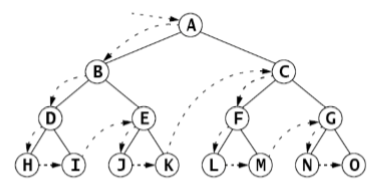
\includegraphics[width=6cm]{pre_order_traversal}
  \caption{Pre-order traversal diagram}
\end{figure}

\subparagraph{In-order traversal}
Visit the left subtree, visit the root, visit the right subtree.

\begin{figure}[H]
  \centering
  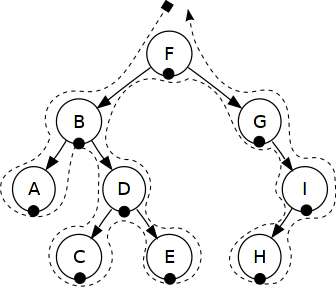
\includegraphics[width=6cm]{in_order_traversal}
  \caption{In-order traversal diagram}
\end{figure}

\subparagraph{Post-order traversal}
Visit the left subtree, visit the right subtree, visit the root.

\begin{figure}[H]
  \centering
  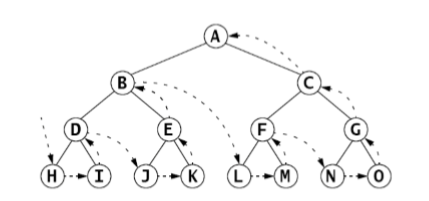
\includegraphics[width=6cm]{post_order_traversal}
  \caption{Post-order traversal diagram}
\end{figure}


\newpage


\paragraph{Insert}
The {\em insert} operation is used to insert new keys into the tree. This is a linear time (\(O(n)\)) operation.
Since the binary search tree property must be maintained, the insert operation has to intelligently locate the
correct position for the new element. The insert operation always starts from the root of the tree,
which may be empty. If the current node is not empty, the algorithm will continue on the left subtree if
the value to be inserted is less than the value in the current key. Otherwise, it will continue on the right
subtree. This process is repeated until an empty node is found. When it is found, the new element will populate
the empty node.

\paragraph{Delete}
The {\em delete} operation is used to delete existing keys from the tree. This is a linear time (\(O(n)\))
operation. First, the element to be deleted must be located. Once the target key is found, the algorithm must
establish how to proceed with the deletion. If the node to be deleted does not have any children, the delete
operation is trivial, as the current node can simply be erased. If the node has a single child, that child will
take the place of the node to be deleted. A more complex situation occurs if the node has two children, as the
binary search tree property must be maintained. To do this, the algorithm must either locate the
{\em in-order successor} or {\em in-order predecessor} of the target node. The located node's key then replaces
the deletion target node's key. After this, the delete operation continues on the located node until one of the
trivial cases occurs.

\paragraph{Search}
The {\em search} operation is a linear time (\(O(n)\)) operation that finds a target node based on its key.
Since the binary search tree property holds, the search operation may from any key easily determine whether to
branch the search operation to the left or right of said node. If an empty node is encountered, the key is
not in the tree.

\paragraph{Sources}
Binary search tree implementations are provided at the following locations:
\begin{itemize}
\item{{\em csharp/data\_structures/binary\_search\_tree/}}
\item{{\em python\_3/data\_structures/}}
\item{{\em bonus/c/data\_structures/}}
\item{{\em bonus/fsharp/data\_structures/}}
\end{itemize}


\subsubsection{K-dimensional tree}
The {\em K-dimensional} tree expands upon the philosophy of the binary search tree, in that it
must maintain a sorting order property. When using this tree in less than 4 dimensions,
a simple geometric interpretation of its structure is possible. Beyond this, the analogy becomes
more difficult to grasp as it involves the splitting of hyperplanes.

\paragraph{Insert}
The {\em insert} operation of a K-dimensional tree is of linear time (\(O(n)\)).
Let's examine the construction of a {\em 2-dimensional} tree from the array \(A = [(3, 2), (6, 5), (7, 1)]\).
The root key of the tree will be the first element in the array, in this case \((3, 2)\).
We will record this key as a {\em vertical} split of the plane, like so:

\begin{figure}[H]
  \centering
  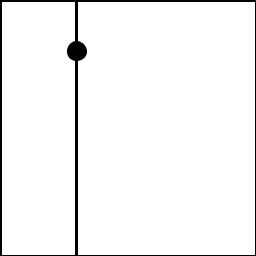
\includegraphics[width=4cm]{2d_tree_0}
  \caption{Node \((3, 2)\) is splitting the plane vertically}
\end{figure}

Since the next key in the collection - \((6, 5)\) - has a larger \(X\) coordinate than the root key(\(6 > 3\)),
it will be stored to the left of the root key. Notice that this operation has added a new level to our tree.
In a 2-dimensional tree each level of the tree will be recorded as being either {\em vertical} or {\em horizontal}.
For this example, let's assume that even levels are vertical, whereas odd levels are horizontal.

\begin{figure}[H]
  \centering
  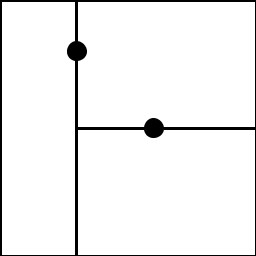
\includegraphics[width=4cm]{2d_tree_1}
  \caption{Node \((6, 5)\) is splitting the subsection of the plane horizontally}
\end{figure}

The next key in our collection - \((7, 1)\) - has a larger \(X\) coordinate than our root key(\(7 > 3\)),
and so the key must be stored in the right subtree. The right subtree is not empty,
therefore we must compare the right child of the root key to the key we're inserting.
Since the right child of the root key is on an odd level in our tree, it corresponds to a {\em horizontal} split.
The consequence of this difference is that we must now compare the \(Y\) coordinates - rather than the \(X\)
coordinates - of our keys. Since the \(Y\) coordinate of our insertion key is less than that of the right child
of the root key, we must store our new element to the left of the right child of the root key.

\begin{figure}[H]
  \centering
  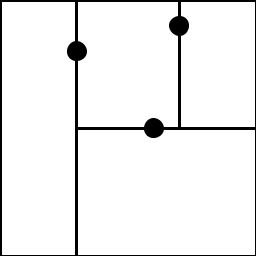
\includegraphics[width=4cm]{2d_tree_2}
  \caption{Node \((7, 1)\) is making yet another vertical split}
\end{figure}

\paragraph{Search}
The {\em search} operation for a key on a k-dimensional tree is of linear time (\(O(n)\)).
When searching for a key, the orientation of each level must be taken into account.
Similar to the insertion operation, the \(X\) or \(Y\) coordinates will be compared to determine
whether the left or right subtree is to be used for the rest of the search operation.
If they key is encountered, the search is succesful. If an empty tree is encountered instead,
the search was not succesful as the key is not in the tree.

\paragraph{Range query}
The {\em range query} operation is of \(O(\sqrt{n} + k)\) time complexity, where \(k\) denotes the number of
reported points. In the 2-dimensional tree, this operation queries a rectangular section of the plane and
returns the points contained within that section.

\begin{figure}[H]
  \centering
  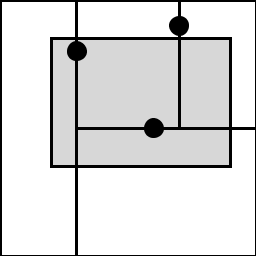
\includegraphics[width=4cm]{2d_tree_3}
  \caption{A range query is performed on the rectangular area \((2, 1.5, 9, 6.5)\)}
\end{figure}

As with the operation that searches for a single key, the range query must take notice of the orientation
associated with each level. Rather than always continuing the query on a single child tree,
the range query may continue on both children if the section covers space on both sides of the current key's split.

\paragraph{Sources}
A K-dimensional search tree implementation is provided at the following location:
\begin{itemize}
\item{{\em csharp/data\_structures/kd\_tree/}}
\end{itemize}


\newpage


\subsection{Graph}
The {\em graph} may be used to represent a relational network of nodes called {\em vertices}.
Vertices are connected via {\em edges}. Vertices that are connected to each other via a single edge are called
{\em adjacent} or {\em neighbors}. A collection of edges connecting two vertices is a {\em path}. The graph does
not imply any particular root, nor does it restrict the number of edges connecting any vertex to other vertices.

\subsubsection{Weighted}
A graph is {\em weighted} if each of its edges has a 'cost' associated with traversing it.
Such graphs may, for instance, be used to map distances between locations on a map.

\subsubsection{Directed}
A graph is {\em directed} if each of its edges has an associated direction. This direction implies a restriction
on the traversal, as only the direction given for each edge is allowed to be travelled. A directed graph is also
called a {\em digraph}.

\subsubsection{Dense versus sparse}
Graphs are called {\em dense} if there are many edges connecting many vertices.
Conversely, a graph may be called {\em sparse} if there are comparatively little edges connecting the vertices.

\subsubsection{Adjacency list}
Graphs may be structured as an {\em adjacency list}. This is a list of vertices, each of which is associated with
all of its neighbors.

% ATTENTION REQUIRED: INCLUDE THE GRAPH?
\begin{figure}[H]
  \centering
  \begin{tabular}{|c|c c c|}
    \hline
    A  & B & C & D  \\ [0.5ex]
    \hline
    B  & A & D & \  \\
    \hline
    C  & D & A & \  \\
    \hline
    D  & C & B & A  \\
    \hline
  \end{tabular}
  \quad
  \begin{tabular}{|c|c c|}
    \hline
    A  & B & D  \\ [0.5ex]
    \hline
    B  & D & \  \\
    \hline
    C  & A & \  \\
    \hline
    D  & C & \  \\
    \hline
  \end{tabular}
  \caption{Examples of adjacency lists. The right list is for a digraph}
\end{figure}

The adjacency list is the preferred representation when the graph is sparse.
In a digraph, only edges that {\em emanate} from (start at) the vertex are recorded for that vertex.

\subsubsection{Adjacency matrix}
The {\em adjacency matrix} is a multi-dimensional array. The axes both contain each vertex in the graph.
If two vertices are adjacent, it is recorded in the matrix. The recorded value may be a boolean type, in which
case the value is \(true\) if the vertices are adjacent. If the graph is weighted, the value may contain the
weight of the connecting edge instead of the boolean value. In this case, the weight for non-adjacent vertices
could be recorded as being infinite.

% ATTENTION REQUIRED: INCLUDE THE GRAPH?
\begin{figure}[H]
  \centering
  \begin{tabular}{|c|c|c|c|c|}
    \hline
    \  & A & B & C & D \\ [0.5ex] 
    \hline
    A  & F & T & T & T \\ 
    \hline
    B  & T & F & F & T \\
    \hline
    C  & T & F & F & T \\
    \hline
    D  & T & T & T & F \\
    \hline
  \end{tabular}
  % ATTENTION REQUIRED: NO WEIGHTS IN THE WEIGHTED MATRIX... Digraphs?
  \quad
  \begin{tabular}{|c|c|c|c|c|}
    \hline
    \  & A & B & C & D \\ [0.5ex] 
    \hline
    A  & \(\infty\) & T & T & T \\ 
    \hline
    B  & T & \(\infty\) & \(\infty\) & T \\
    \hline
    C  & T & \(\infty\) & \(\infty\) & T \\
    \hline
    D  & T & T & T & \(\infty\) \\
    \hline
  \end{tabular}
  \caption{Examples of adjacency matrices. The right matrix is for a weighted graph}
\end{figure}

The adjacency matrix is the preferred representation when the graph is dense.

\subsubsection{Incidence matrix}
The {\em incidence matrix} shows the relationship between vertices (represented in the rows) and edges
(represented in the columns) in a graph. If the vertices are incident upon (connected to) the edge, a boolean
value or weight may be recorded in the matrix.

% ATTENTION REQUIRED: INCLUDE THE GRAPH?
\begin{figure}[H]
  \centering
  \begin{tabular}{|c|c|c|c|c|}
    \hline
    \  & 0 & 1 & 2 & 3 \\ [0.5ex]
    \hline
    0  & F & T & T & T \\ 
    \hline
    1  & T & F & F & T \\
    \hline
    2  & T & F & F & T \\
    \hline
    3  & T & T & T & F \\
    \hline
  \end{tabular}
  \quad
  %ATTENTION REQUIRED: WEIGHTS ARE WRONG ... Digraphs?
  \begin{tabular}{|c|c|c|c|c|}
    \hline
    \  & 0 & 1 & 2 & 3 \\ [0.5ex]
    \hline
    0  & \(\infty\) & T & T & T \\
    \hline
    1  & T & \(\infty\) & \(\infty\) & T \\
    \hline
    2  & T & \(\infty\) & \(\infty\) & T \\
    \hline
    3  & T & T & T & \(\infty\) \\
    \hline
  \end{tabular}
  \caption{Examples of incidence matrices. The right matrix is for a weighted digraph}
\end{figure}

In a digraph, edges that emanate from the row vertex are given the value 1. Edges that terminate at the row vertex
are instead given the value -1.

\subsubsection{Traversal}
Here are listed two ways to visit each vertex in a graph,
both of which are of linear time (\(O(n)\)) complexity.

\paragraph{Breadth-first search}
The {\em breadth-first search} uses the {\em queue} data structure. The general procedure is as follows:
\begin{enumerate}
\item{Enqueue the root vertex}
\item{Dequeue a vertex. If this is the target, stop the search. Otherwise, enqueue all unvisited direct children}
\item{If the queue is empty, the traversal is complete and the search was unsuccesful. Otherwise repeat step 2}
\end{enumerate}

% ATTENTION REQUIRED: INCLUDE GRAPHIC

\paragraph{Depth-first search}
The {\em depth-first traversal} uses the {\em stack} data structure. The general procedure is as follows:
\begin{enumerate}
\item{Start at the root vertex}
\item{If the current vertex is the target, stop the search. Otherwise, continue at step 3}
\item{Push the first unvisited neighboring vertex onto the stack}
\item{Repeat step 3 until no more unvisited neighbors exist, then pop from the stack. Repeat from step 2}
\end{enumerate}

% ATTENTION REQUIRED: INCLUDE GRAPHIC


\newpage


\section{Algorithms}
\subsection{Searching}
\subsubsection{Linear search}
The {\em linear search} traverses a collection in linear fashion until either the requested element is found,
or the end of the collection was reached. This is a linear time (\(O(n)\)) operation.
Linear search is simple to implement and is well-suited to small unsorted collections.

\paragraph{Sources}
Linear search implementations are provided at the following locations:
\begin{itemize}
\item{{\em csharp/algorithms/searching/}}
\item{{\em python\_3/algorithms/}}
\item{{\em bonus/c/algorithms/}}
\item{{\em bonus/fsharp/algorithms/}}
\item{{\em bonus/rust/searching/}}
\item{{\em bonus/chicken\_scheme/algorithms/}}
\end{itemize}

\subsubsection{Binary search}
If the collection is known to be sorted, the {\em binary search} algorithm may yield a significant performance
gain compared to regular insertion sort. This is because the algorithm can use a pivot to intelligently search
the collection. This is a logarithmic time (\(O(log n)\)) operation.

% ATTENTION REQUIRED: RATHER SPARSE DESCRIPTION OF THE ALGORITHM

\paragraph{Sources}
\begin{itemize}
\item{{\em csharp/algorithms/searching/}}
\item{{\em python\_3/algorithms/}}
\item{{\em bonus/rust/algorithms/searching/}}
\end{itemize}


\newpage


\subsection{Sorting}
Here are described various sorting algorithms of which I have provided implementations in various programming
languages.

\subsubsection{Insertion sort}
Perhaps the most basic sorting algorithm is {\em insertion sort}. Insertion sort must in the worst case compare
each element to every other element in the collection. It is therefore of quadratic time (\(O(n^2)\)) complexity.
The process is frequently compared to the steps involved in sorting a hand of playing cards.

\paragraph{Setup}
This algorithm expects as input a linear collection of sortable keys.

\paragraph{Process}
For each element in the collection:
\begin{enumerate}
\item{If the key has a left-side neighbor, compare it to that neighbor}
\item{If the key is smaller than its neighbor, swap them}
\item{Repeat from step 1 until either no more neighbor exists, or the key is larger than its neighbor}
\end{enumerate}

\paragraph{Sources}
\begin{itemize}
\item{{\em csharp/algorithms/searching/}}
\item{{\em python\_3/algorithms/}}
\item{{\em bonus/fsharp/algorithms/}}
\item{{\em bonus/rust/algorithms/searching/}}
\end{itemize}

\subsubsection{Shell sort}
The {\em shell sort} algorithm utilizes insertion sort in a {\em divide-and-conquer} strategy.
Shell sort is a \(O(n log^2 n)\) time complexity algorithm.

\paragraph{Setup}
The algorithm expects as inputs a collection of sortable keys and a slice size. The collection will be cut up into
slices according to the provided size. The results are stored into a buffer list or array.

\paragraph{Process}
\begin{enumerate}
\item{For each slice:}
  \begin{enumerate}
  \item{Run insertion sort on the slice}
  \item{Once complete, concatenate the sorted slice to the buffer}
  \end{enumerate}
\item{Run insertion sort on the buffer}
\end{enumerate}

\paragraph{Sources}
\begin{itemize}
\item{{\em csharp/algorithms/shell\_sort/}}
\item{{\em python\_3/algorithms/}}
\end{itemize}


\subsubsection{Bubble sort}
The {\em bubble sort} algorithm lets elements in an unsorted collection 'bubble' up to the correctly sorted position
in the resulting collection. Bubble sort is of quadratic time (\(O(n^2)\)) complexity.

\paragraph{Setup}
The algorithm expects as input an unsorted collection. It keeps track of an index indicating how many keys are
already sorted.

\paragraph{Process}
Until no more swaps are necessary:
\begin{enumerate}
\item{Take a slice from the index to the end of the collection and increment the index}
\item{Take the rightmost key from the slice}
\item{If the key does not have a left-side neighbor, the algorithm is complete}
\item{If the left-side neighbor is smaller than the key, swap the keys. Otherwise, continue from step 1}
\item{Repeat from step 1 until the algorithm is finished}
\end{enumerate}

\paragraph{Sources}
\begin{itemize}
\item{{\em csharp/algorithms/bubble\_sort/}}
\item{{\em python\_3/algorithms/}}
\end{itemize}


\subsubsection{Comb sort}
The {\em comb sort} algorithm addresses a problem with bubble sort % WHAT PROBLEM?

\paragraph{Sources}
\begin{itemize}
\item{{\em csharp/algorithms/comb\_sort/}}
\item{{\em python\_3/algorithms/}}
\end{itemize}


\iffalse
% ATTENTION REQUIRED: RADIX SORT IS MISSING? DID I FORGET TO ADD IT TO THE REPOSITORY?
\subsubsection{Radix sort}
\paragraph{Sources}
\begin{itemize}
\item{{\em python\_3/algorithms/}}
\end{itemize}
\fi

\subsubsection{Counting sort}
\paragraph{Sources}
\begin{itemize}
\item{{\em csharp/algorithms/counting\_sort/}}
\item{{\em python\_3/algorithms/}}
\end{itemize}


\subsubsection{Bucket sort}
\paragraph{Sources}
\begin{itemize}
\item{{\em csharp/algorithms/bucket\_sort/}}
\item{{\em python\_3/algorithms/}}
\end{itemize}


\subsubsection{Heap sort}
\paragraph{Sources}
\begin{itemize}
\item{{\em csharp/algorithms/heap\_sort/}}
\item{{\em python\_3/algorithms/}}
\end{itemize}


\subsubsection{Merge sort}
This sorting algorithm splits a collection into many small collections.
Each of these small collections is sorted and subsequently merged with another small collection.
Eventually this algorithm yields a sorted collection faster than a regular insertion sort.

\paragraph{Sources}
\begin{itemize}
\item{{\em csharp/algorithms/merge\_sort/}}
\item{{\em python\_3/algorithms/}}
\item{{\em bonus/c/algorithms/}}
\end{itemize}


\subsubsection{Quick sort}
Via the use of a pivot, the collection is divided and subsequently conquered.

\paragraph{Sources}
\begin{itemize}
\item{{\em csharp/algorithms/quick\_sort/}}
\item{{\em python\_3/algorithms/}}
\end{itemize}


\subsubsection{Monkey sort}
Imagine having an unsorted deck of cards, then throwing it in the air and picking it up to see if the new distribution is sorted.
If it's not, then you repeat the process. This is a quaint description of {\em Monkey sort}.
It's a highly inefficient sorting algorithm, in which a random distribution of the collection is made every time.
Subsequently, the new distribution goes through a process that verifies if it is sorted. If it is not sorted, a new distribution is made.
Since this algorithm may never yield a sorted distribution, the complexity is unbounded (\(O(\infty)\)).

\paragraph{Sources}
\begin{itemize}
\item{{\em python\_3/algorithms/}}
\end{itemize}


\newpage


\subsection{Shortest path determination}
In this section, each of the following algorithms is assumed to operate on the following graph:

\begin{figure}[H]
  \centering
  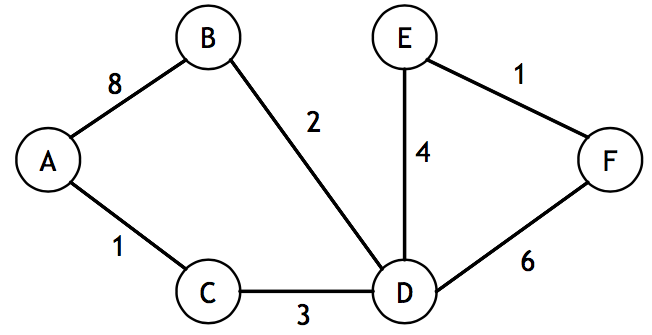
\includegraphics[width=6cm]{sample_graph}
  \caption{A weighted graph}
\end{figure}

When recording this graph as data, letters are replaced with 0-based indices, such that \(A=0, B=1, C=2, \dots\).


% ATTENTION REQUIRED: Graphics would be nice
\subsubsection{Dijkstra}
{\em Dijkstra's} algorithm finds all shortest path distances between a {\em source} vertex and all other vertices
in a graph. Dijkstra's algorithm runs in quadratic time (\(O(n^2)\)). It's possible to optimize Dijkstra's algorithm
using a {\em Fibonacci heap} as a priority queue, although my implementation does not include one.

\paragraph{Setup}
The algorithm accepts as inputs a graph and a source vertex. First it sets up an array which will hold the result
distances. This array is initially populated with the value \(\infty\), with the exception of the source vertex's
distance to itself; which is 0.

\paragraph{Process}
All unvisited vertices are stored in a list, so that the algorithm may prevent itself from repeatedly
processing previously visited vertices. As long as unvisited vertices remain, the algorithm will select the closest
unvisited vertex and remove it from the list of unvisited vertices. For each neighboring vertex, the algorithm will
check if the newly found distance to it is smaller than the currently recorded vertex. If it is, the new distance
will be recorded in the distances array. When no unvisited vertices remain, the distances array will be populated
with all shortest path distances.

\paragraph{Chain}
With a slight modification it becomes possible to also track the actual paths, rather than just the distances.
During the setup phase, the algorithm should also create an array which will hold the chain information.
Initially, all values will be set to null. Whenever a shorter distance is found, the current vertex will be
recorded in the chain using the neighbor's ID as the index.

\subparagraph{Shortest path}
The {\em shortest path} operation can compute the actual shortest path when given two vertex ID's and a precomputed
chain. It is a linear time (\(O(n)\)) algorithm. The result of the shortest path operation will be a list containing
each step of the path. The operation starts at the target vertex. As long as the currently inspected vertex is not
null, it is appended to the existing path. The next vertex to inspect may be located by using the current vertex ID
as the index of the next path vertex in the chain.

\paragraph{Sources}
Floyd-Warshall implementations are provided at the following locations:
\begin{itemize}
\item{{\em csharp/algorithms/dijkstra/}}
\item{{\em python\_3/algorithms/}}
\end{itemize}


% ATTENTION REQUIRED: GRAPHICS WOULD BE NICE
\subsubsection{Floyd-Warshall}
Rather than Dijkstra's focus on a single source, {\em Floyd-Warshall} finds the shortest path between each vertex
and all other vertices in a graph. Unlike Dijkstra's algorithm, Floyd-Warshall supports negative weights.
Initially one might suspect that this algorithm somehow runs Dijkstra on each vertex, which would be rather
inefficient. Fortunately, Floyd-Warshall uses a more clever approach.

\paragraph{Setup}
The algorithm expects a graph, which I've provided in the form of a weighted adjacency list. An initial 'guess' is
prepared by setting up a matrix of distances between vertices in the graph. This matrix will at first contain the
value \(\infty\) for each distance. To improve the initial guess, the matrix is populated with the known distances
between adjacent vertices.

\paragraph{Process}
There are three nested {\em for} loops, using the variables \(i\), \(j\), and \(k\). At each iteration,
\(i\) and \(j\) are two vertices between which the algorithm is trying to find the shortest path. The most important
aspect of the algorithm actually relies on \(k\). At each iteration, \(k\) represents a vertex between \(i\) and
\(j\) that potentially yields a shorter path from \(i\) to \(j\). This means that each time we find a shorter path,
we'll have to update the currently recorded value in our distance matrix. Since we have three nested {\em for} loops
that each scale according to the amount of vertices in the graph, it naturally follows that our algorithm is of
cubic time (\(O(n^3)\)) complexity.

\paragraph{Sources}
Floyd-Warshall implementations are provided at the following locations:
\begin{itemize}
\item{{\em csharp/algorithms/floyd\_warshall/}}
\item{{\em python\_3/algorithms/}}
\end{itemize}


\newpage



\iffalse



\section{Advanced C\# features}
% ATTENTION REQUIRED: MARKED FOR SCRAPPING, VERY MUCH INCOMPLETE
\subsection{Properties}
This concept allows the programmer to specify how data inside a class may be accessed.
With this feature, manually writing {\em get} and {\em set} functions becomes obsolete.

\subsection{Interfaces}
Interfaces are contracts that guarantee a class implements certain methods.

\subsection{Events}


\subsection{Extension methods}
In order to extend the functionality offered by base types, a programmer may use extension methods.

\subsection{Lambdas, delegates and higher order functions}
Higher order functions are part of what makes functional programming so powerful.
In C\#, delegates and lambdas offer the features required for higher order functions.

Here are several examples of how these concepts may be applied.

\paragraph{Iter}
This operation iterates over a sequence of elements. For each of these elements the provided lambda will be executed.

\begin{lstlisting}[language=Python]
  // This function prints all elements in the collection
  List.iter (fun element -> printfn "%A" element) collection
\end{lstlisting}

\paragraph{Filter}
This operation iterates over a sequence of elements. For each of these elements, the provided lambda predicate will be executed.
Elements for which this predicate returns True will be in the resulting list. Contrastingly, elements for which the predicate returns False will be discarded.

\begin{lstlisting}[language=Python]
  // This function returns all elements in the collection that are even
  List.filter (fun element -> element % 2 == 0) collection
\end{lstlisting}

\paragraph{Map and reduce}
This operation iterates over a sequence of elements. For each of these elements, the provided lambda will be executed.
The lambda contains a function that manipulates the current element. The result of this operation is the list of transformed elements.

\begin{lstlisting}[language=Python]
  //This function returns all transformed elements in the collection
  List.map (fun element -> element + 4) collection
\end{lstlisting}
  
\paragraph{Fold}

\paragraph{LINQ}


\subsection{Anonymous types}
Using this feature, programmers may easily specify new types with a comfortable syntax.

\begin{lstlisting}[language=Python]
  var some_type = { SomeProperty = 5 };
\end{lstlisting}

\subsection{Iterators and state machines}


\subsection{Indexers and enumerators}

\newpage

\section{Asynchronous programming}
\subsection{Async and await}
\subsection{Coroutines}
\subsubsection{The coroutine monad}
\subsection{Threading}

\newpage

\section{Design patterns}

\subsection{Option and Visitor}
These design patterns when combined form a great answer to the infamous null-reference-exception.
In essence, the {\em option} pattern offers a syntactical construct that forces the programmer to deal with missing data at {\em compile time}.
Data in the option is said to be either {\em some data} or {\em none}, the latter of which replaces the traditional {\em null}.
Since {\em none} is {\em no data} rather than {\em missing data}, a null-reference-exception shan't occur.

The option's counterpart is the {\em visitor}, which offers a syntactical construct to perform different operations depending on whether data
is missing({\em none}) or readily available ({\em some data}).

The following example demonstrates this process:

\begin{lstlisting}[language=Python]
\end{lstlisting}

The two variables({\em noneData} and {\em someData}) are defined to be of type {\em Option String}.
That is to say, the variables may either hold actual data({\em some}) or not{\em none}.
When interacting with {\em Option} data, the programmer must use a {\em match} expression.
Such an expression is forced by the compiler to deal with both possible cases({\em some} and {\em none}.
Notice how {\em some} comes with a {\em data} object, {\em none} does not.

\subsection{Factory}
\subsection{Strategy}
The strategy pattern is used where different strategies may be optimal depending on context.
For instance, if we know a collection to be mostly sorted, we might choose to use a different sorting algorithm than when the collection is mostly unsorted.


\subsection{Adapter}
Programmers will frequently encounter situations in which they must deal with error-prone code.

Unfortunately, one is frequently not allowed to modify existing code.
To deal with this situation efficiently, the programmer may employ a technique called the {\em adapter pattern}.
The adapter pattern consists of building a new interface to existing code.
The primary purpose of this new interface is to guarantee proper interaction with the existing code.

\newpage

\section{Conclusion}
% Something about mathematical proofs, more data structures / algorithms, set theory / category theory

% ATTENTION REQUIRED: INCOMPLETE SECTION
\section{Thanks}
I'd like to especially thank the following people for supporting me in my research:
\begin{itemize}
\item{Giuseppe Maggiore}
\item{Mohamed Abbadi}
\item{Francesco di Giacomo}
\item{Giulia }
\item{Fernando Cabello Domingo}
\item{}
\end{itemize}

\section{Bibliography}


\fi


\end{document}
